\newpage
\section{TGGs in action}
\genHeader
\label{sect:TGGs_in_Action}
In this section, we shall export our TGG, implement our new constraint, and get our integration running! The instructions for both syntaxes are virtually the
same, but keep a lookout for colored bullet arrows regarding syntax-specific commands

\vspace{0.5cm}

\begin{itemize}
\item[\color{RedOrange}$\blacktriangleright$] Export your metamodels and TGG from EA by choosing ``\texttt{Extensions/\-MOFLON::\-Ecore Addin\-/Export all to
Workspace}' and refresh your Eclipse metamodel project.

\vspace{0.5cm}

\item[\color{CornflowerBlue}$\blacktriangleright$] Go to the toolbar and press \texttt{Build (without cleaning)}, and make sure your metamodel project
refreshes.
\end{itemize}

\vspace{0.5cm}

If you have done everything right, code generation and compilation should terminate without error, and the structure of the \texttt{gen} folder in
\texttt{LearningBox\-To\-Dictionary\-Integration} should resemble Fig.~\ref{fig:gen_folder}.

\begin{figure}[htbp]
\begin{center}
  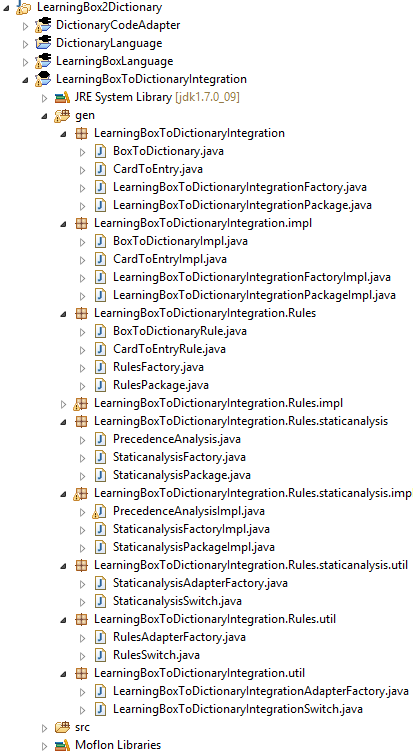
\includegraphics[width=0.8\textwidth]{tgg22}
  \caption{Integration project after code generation}
  \label{fig:gen_folder}
\end{center}
\end{figure}

\begin{itemize}

\vspace{0.5cm}
  
\item[$\blacktriangleright$] To implement the \texttt{IndexToLevel} constraint, locate and open the file \texttt{csp/IndexToLevel.java} under
  ``LearningBoxToDictionaryIntegration/src/'' 

\vspace{0.5cm}
  
\item[$\blacktriangleright$] Copy and paste the code provided in Fig.~\ref{fig:indexToLevel} into the file.

\end{itemize}

\begin{figure}[htbp]
\begin{center}
  % 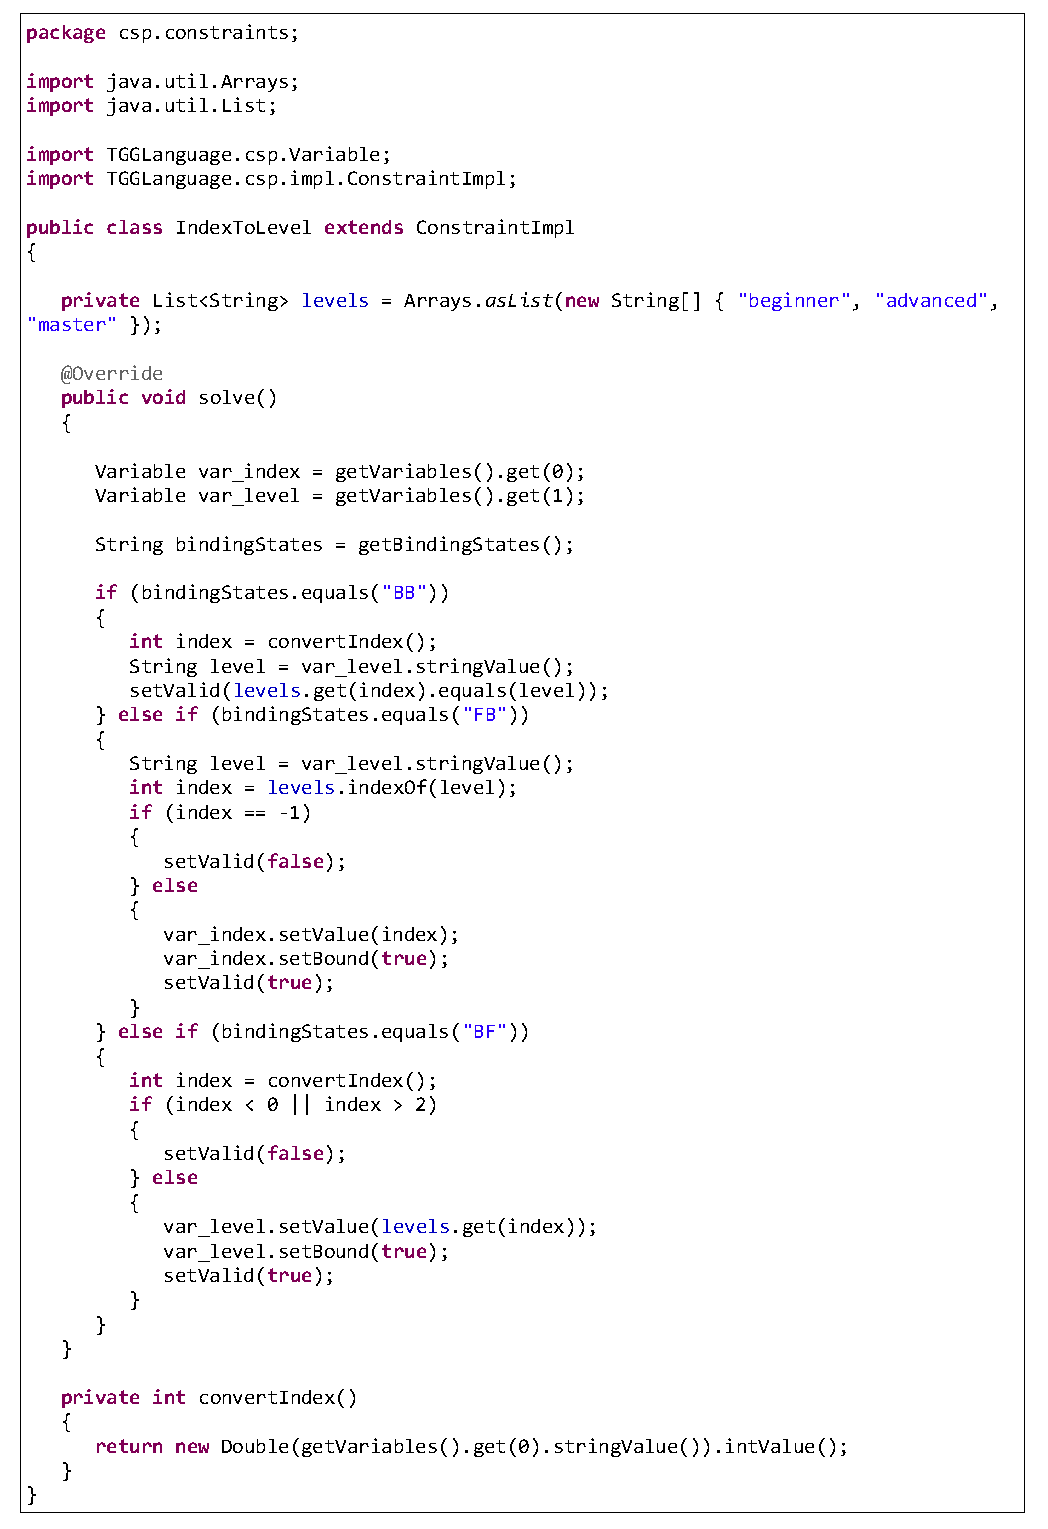
\includegraphics[height=0.64\textheight]{pics/tggBilder/transformation/tgg23}
\begin{lstlisting}[language=Java,backgroundcolor=\color{white}, keywordstyle={\bfseries\color{purple}}]
package csp.constraints;

import java.util.Arrays;
import java.util.List;

import TGGLanguage.csp.Variable;
import TGGLanguage.csp.impl.ConstraintImpl;

public class IndexToLevel extends ConstraintImpl {

  private List<String> levels = Arrays.asList(new String[] { "beginner",
      "advanced", "master" });


  public void solve(Variable<Integer> var_0, Variable<String> var_1){
    String bindingStates = getBindingStates(var_0, var_1);

    switch(bindingStates){
    case "BB":
      int indexBB = var_0.getValue().intValue();
      String level = var_1.getValue();
      setSatisfied(levels.get(indexBB).equals(level));
      break;
    case "BF":
     int indexFB = var_0.getValue().intValue();
      if (indexFB < 0 || indexFB > 2) {
        setSatisfied(false);
      } else {
        var_1.setValue(levels.get(indexFB));
        var_1.setBound(true);
        setSatisfied(true);
      }
      break;
    case "FB":
      String levelBF = var_1.getValue();
      int indexBF = levels.indexOf(levelBF);
      if (indexBF == -1) {
        setSatisfied(false);
      } else {
        var_0.setValue(indexBF);
        var_0.setBound(true);
        setSatisfied(true);
      }
      break;
    }

  }
}
\end{lstlisting}
  \caption{Implementation of our attribute constraint}
  \label{fig:indexToLevel}
\end{center}
\end{figure}

\clearpage

Now we shall create an instance model\footnote{Refer to Part II, Section 3 for review} of one of our languages, then transform it into an instance model of the
\emph{other} language as according to our TGG (i.e., perform a forward and backward transformation). Since dictionaries are a much simpler structure, lets start
with the ``backwards''\footnote{No direction implied} transformation, dictionary to learning box.

\begin{itemize}
\item[$\blacktriangleright$] Navigate to and open \texttt{Dictionary\-Language/model/Dictionary\-Language.ecore}. Create a dynamic instance of
\texttt{Dictionary} named \texttt{target.xmi}, and save it under \texttt{Learn\-ing\-Box\-To\-Dictionary\-In\-te\-gra\-tion/in\-stan\-ces/}
(Fig.~\ref{fig:create_instance_dict}).

\begin{figure}[htbp]
\begin{center}
  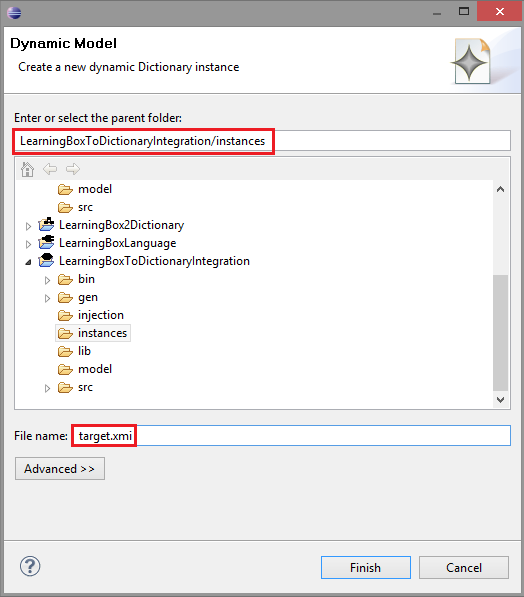
\includegraphics[width=0.7\textwidth]{tgg24}
  \caption{Create a dynamic instance of \texttt{Dictionary}}
  \label{fig:create_instance_dict}
\end{center}
\end{figure}

\item[$\blacktriangleright$] Open \texttt{target.xmi}, and edit the \texttt{Dictionary} properties by setting \texttt{Title} to \texttt{English Numbers}.

\item[$\blacktriangleright$] Create two child \texttt{Entry} objects. Set \texttt{Content} of the first to \texttt{one : eins} and its
\texttt{Level} as \texttt{beginner}. Set the second with \texttt{eleven : elf} and \texttt{advanced} (Fig.~\ref{fig:dictionaryxmi}).

\begin{figure}[htbp]
\begin{center}
  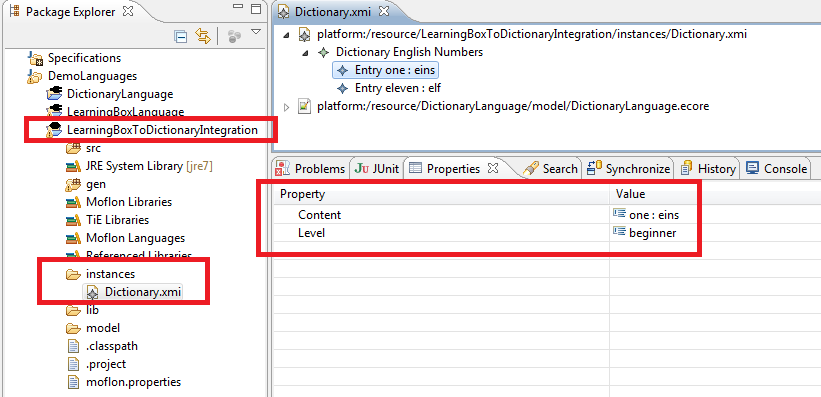
\includegraphics[width=\textwidth]{tgg26}
  \caption{Contents of the dictionary}
  \label{fig:dictionaryxmi}
\end{center}
\end{figure}

\item[$\blacktriangleright$] Run the main class, \texttt{TGGMain}, found in \texttt{LearningBox\-To\-Dictionary\-In\-te\-gra\-tion\-/src}, and refresh
\texttt{LearningBox\-To\-Dictionary\-In\-te\-gra\-tion/\-instances}.

\vspace{0.5cm}

\item[$\blacktriangleright$] Note the console error message, ``Unable to load instances/source.xmi, instances/source.xmi does not exist.'' This is referring to
the non-existent source file for the ``forward'' transformation - we'll fix this in a moment.
\end{itemize}

As you can see, our \texttt{Dictionary} has been translated backward to a \texttt{Box} with the same name (\texttt{English Numbers}) and containing three
\texttt{Par\-ti\-tions} (as specified in \texttt{Box\-To\-Dictionary\-Rule}). The two \texttt{Entry} objects have been translated to \texttt{Card} objects as
specified in \texttt{CartToEntryRule}. The \texttt{face} and the \texttt{back} of the \texttt{Card}s are consistent with the \texttt{content}
of the corresponding \texttt{Entry}, e.g. \texttt{card.face = ``Question : one''} and \texttt{card.back = ``Answer : eins''}. The indices of the partitions
containing the cards are also consistent with the level of the entry, i.e., \texttt{0} for \texttt{beginner}, and \texttt{1} for \texttt{advanced}.

\vspace{0.5cm}

Congratulations! You have successfully performed your first \emph{backward} transformation from your target model (dictionary) to your source (Learning box)
using TGGs! To show that the transformation is actually bidirectional however, lets edit the source model (thus resolving the error from above) and transform it
\emph{forward} to a new target model:

\begin{itemize}
\item[$\blacktriangleright$] Make a copy of \texttt{target.xmi\_BWD.xmi} (the result of the backward transformation)
and rename it to \texttt{source.xmi}.
  
\item[$\blacktriangleright$] Open \texttt{source.xmi} and create some new \texttt{Card} objects in the \texttt{Partition}s (e.g., create a new \texttt{Card}
with \texttt{Card.face = ``Question : two''}, \texttt{Card.back = ``Answer : zwei''} in \texttt{Partition 0}).

\item[$\blacktriangleright$] Run the \texttt{TGGMain.java} again and inspect the result of the forward transformation, target model
\texttt{source.xmi\_FWD.xmi}.

\end{itemize}


To end this chapter on TGGs, lets check out another feature of eMolfon, the integrator visualizer! This will let us view the visualization of the created
triple model.

\newpage

\begin{itemize}

\item[$\blacktriangleright$] Right-click on \texttt{corr\_BWD.xmi} and choose ``eMoflon $\rightarrow$ Start Integrator'' which will open the window depicted in
Fig.~\ref{fig:integrator_start}.

\vspace{0.5cm}

\begin{figure}[htbp]
\begin{center}
  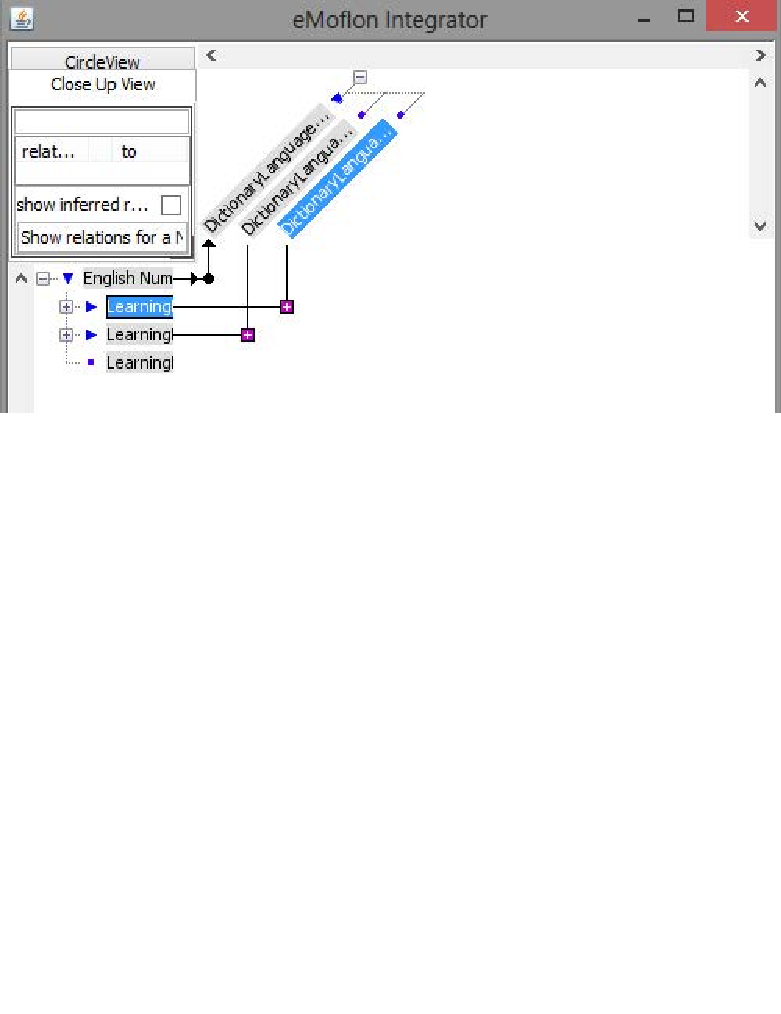
\includegraphics[width=0.7\textwidth]{integrator_start_view.pdf}
  \caption{Default view of the integrator}
  \label{fig:integrator_start}
\end{center}
\end{figure}

\item[$\blacktriangleright$] Drag and drop \texttt{protocol\_BWD.xmi} into the window. You will now see the controls explained in the lower part of the window 
(Fig.~\ref{fig:integrator_after_protocol}).

\begin{figure}[h!]
\begin{center}
  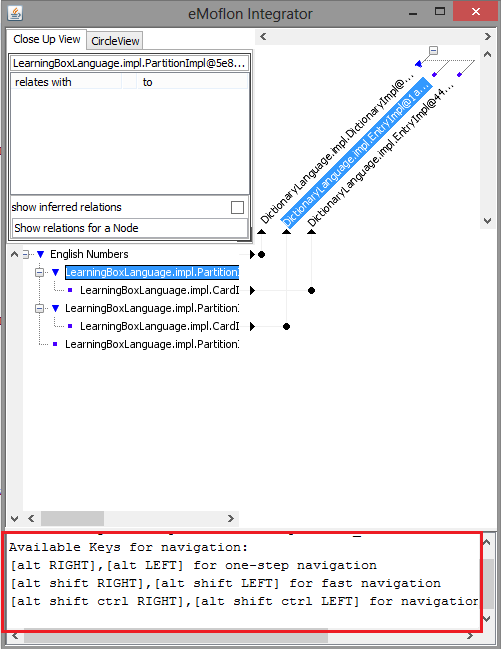
\includegraphics[width=0.6\textwidth]{integrator_after_protocol_insertion.png}
  \caption{Integrator after protocol insertion.}
  \label{fig:integrator_after_protocol}
\end{center}
\end{figure} 
\FloatBarrier

\item[$\blacktriangleright$] The integrator works as an ``offline'' debugger, working on the protocol (trace) of the transformation. You can use
\texttt{Alt+Right} to navigate forwards \emph{through} the transformation process, and \texttt{Alt+Left} to go backwards.  When you step through the
transformation, you will notice that some elements are highlighted with colours. These are the elements currently being processed. The colours have the
following definitions:
\begin{description}
  \item[Blue] The element is now about to be processed (is being ``looked at'').
  \vspace{0.5cm}
  \item[Yellow] The element cannot be transformed right now and has been queued for later transformation 
  (e.g., when transforming an Entry to a Card, the Box with partitions to put the 
  Card into must be translated first).
  \vspace{0.5cm}
  \item[Green] The object has just been created.
\end{description}

\end{itemize}
